\documentclass[titlepage,landscape]{seminar}
\usepackage{url}
\usepackage{graphicx}
\usepackage{hyperref}
\usepackage{epstopdf}
\usepackage{slides}

\newcommand{\frack}{\frac{1}{k}}

\begin{document}

\myslide{
  \heading{Results from Lab \#5}

  \begin{center}
    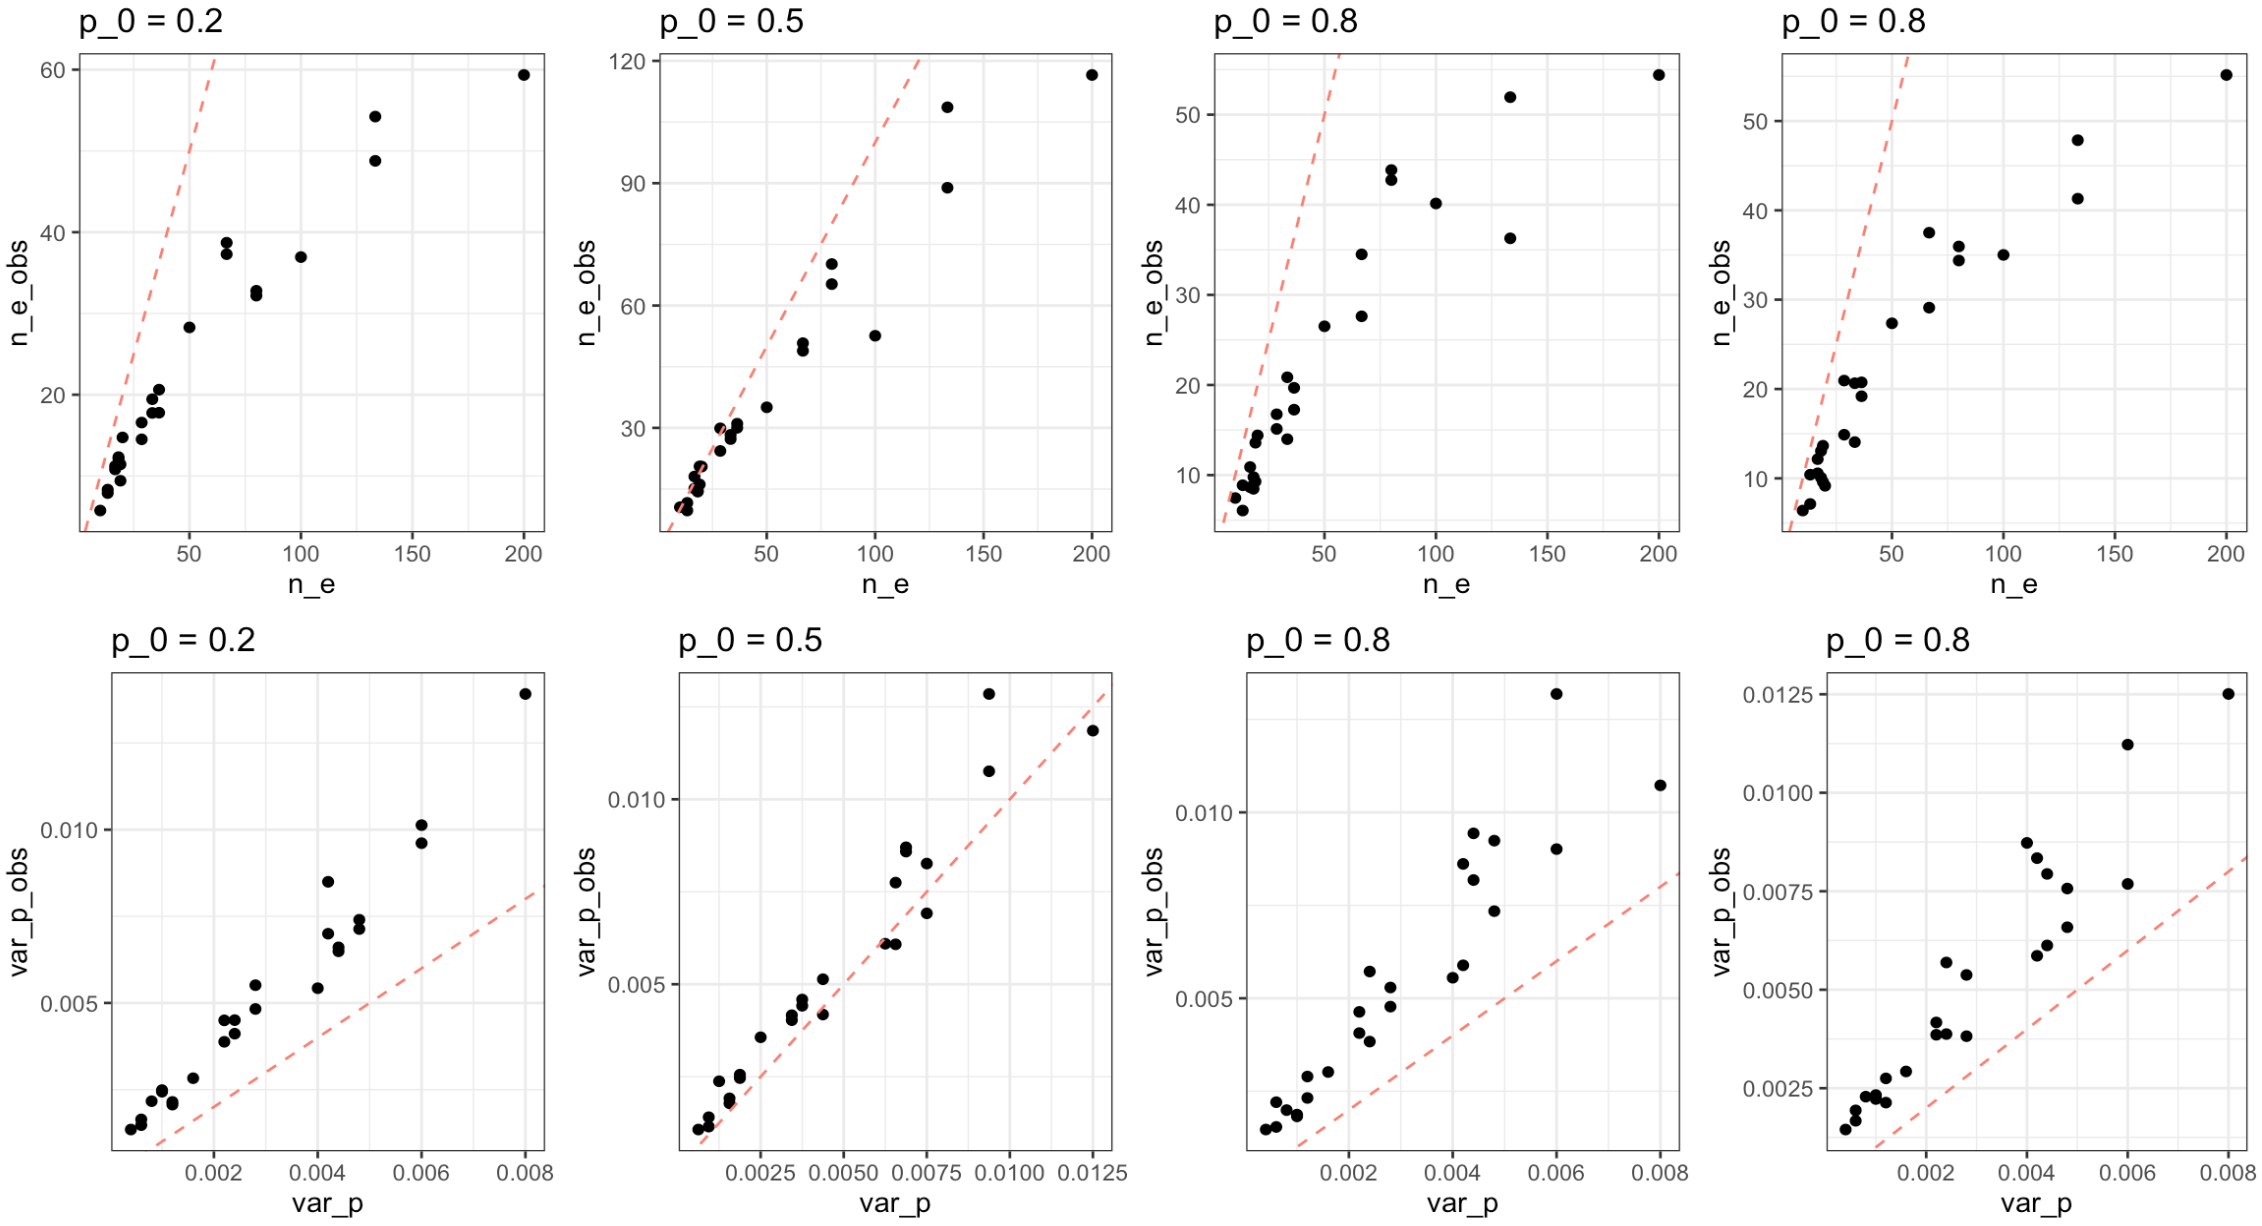
\includegraphics[width=\textwidth]{n_e_simulations.png}
  \end{center}

  \begin{itemize}
    \item $p_0 = 0.2, 0.5$: {\tt n\_samp = n\_pop = 100}
    \item $p_o = 0.8$: {\tt n\_samp = 100}, {\tt n\_pop = 100, 1000}
  \end{itemize}
}

\myslide{
\heading{Genetic drift: Analogy to inbreeding}
\begin{eqnarray*}
f_{t+1} &=& \mbox{Prob. ibd from preceding generation} \\
        &&  + (\mbox{Prob. not ibd from prec. gen.}) \times (\mbox{Prob. ibd from
          earlier gen.}) \\
        && \\
   &=& \frac{1}{2N} + \left(1 - \frac{1}{2N}\right)f_t
\end{eqnarray*}
\[
f_{t+1} = 1 - \left(1 - \frac{1}{2N}\right)^t(1-f_0)
\]
}

\myslide{
\heading{Genetic drift: Variance effective size}
\[
Var(p_{t+1}) = \frac{p_t(1-p_t)}{2N} \quad.
\]
\vfil
\[
N_e^{(v)} = \frac{p(1-p)}{2\widehat{Var}(p)}
\]
}

\myslide{
\heading{Genetic drift: Inbreeding effective size}
\begin{eqnarray*}
f_{t+1} &=& \frac{1}{2N} \quad \mbox{assuming $f_t = 0$} \\
N_e^{(f)} &=& \frac{1}{2\hat f_{t+1}}
\end{eqnarray*}
}

\myslide{
\heading{Effective size: Unequal sex ratio}
\vfill
\[
N_e^{(f)} = \frac{4N_fN_m}{N_f + N_m}
\]
\vfill
}

\myslide{
\heading{Effective size: Variation in population size}
\vfill
\[
N_e^{(f)} \approx \left(\left(\frac{1}{K}\right)
                    \sum_{i=1}^K\frac{1}{N_{t+i}}\right)^{-1}
\]
\vfill
}


\myslide{
\heading{Effective size: Variance in offspring number}
\vfill
\[
N_e^{(f)} = \frac{2N - 1}{1 + \frac{V_k}{2}} \quad ,
\]
\vfill
\begin{itemize}

\item $N_e^{(f)} < N$ if $V_k > 2(1 - 1/N)$ and

\item $N_e^{(f)} > N$ if $V_k < 2(1 - 1/N)$.

\end{itemize}
}

\myslide{
\heading{Drift and mutation}
\vfill
\[
f_{t+1} = \left(\left(\frac{1}{2N}\right) +
          \left(1 - \frac{1}{2N}\right)f_t\right)(1-\mu)^2
\]
\vfill
}

\myslide{
\heading{Drift and mutation}
\begin{eqnarray*}
\hat f &=& \left(\left(\frac{1}{2N}\right) +
          \left(1 - \frac{1}{2N}\right)\hat f\right)(1-\mu)^2 \\
\hat f\left(1 -
\left(1 - \frac{1}{2N}\right)(1-\mu)^2\right)
       &=& \left(\frac{1}{2N}\right)(1-\mu)^2 \\
\hat f &=& \frac{\left(\frac{1}{2N}\right)(1-\mu)^2}
           {1 -\left(1 - \frac{1}{2N}\right)(1-\mu)^2} \\
       &\approx& \frac{1 - 2\mu}
           {2N\left(1 - \left(1 - \frac{1}{2N}\right)(1-2\mu)\right)} \\
       &=& \frac{1 - 2\mu}
           {2N\left(1 - 1 + \frac{1}{2N} + 2\mu -
            \frac{2\mu}{2N}\right)} \\
       &=& \frac{1 - 2\mu}{1 + 4N\mu - 2\mu} \\
       &\approx& \frac{1}{4N\mu + 1}
\end{eqnarray*}
}

\myslide{
\heading{Drift and mutation}
\begin{center}
\resizebox{!}{0.9\textheight}{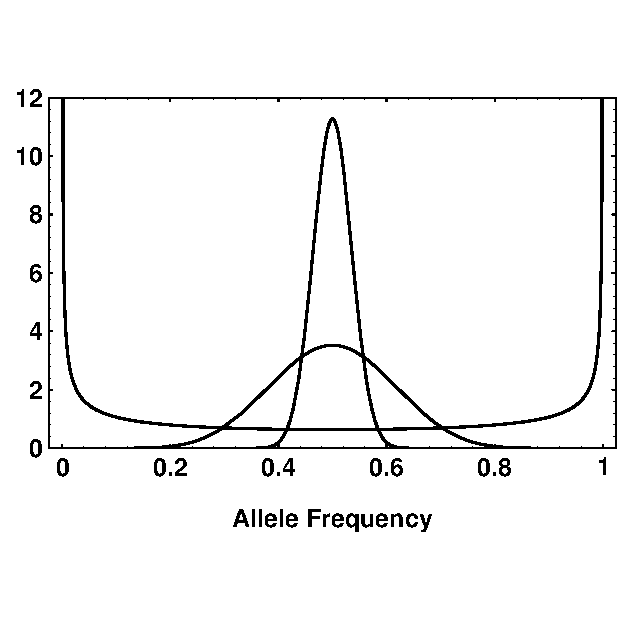
\includegraphics{mutation.eps}}
\end{center}
}

\myslide{
\heading{Drift and migration}
\vfill
\[
f_{t+1} = \left(\left(\frac{1}{2N}\right) +
          \left(1 - \frac{1}{2N}\right)f_t\right)(1-m)^2
\]
\vfill
\[
\hat f \approx \frac{1}{4Nm + 1}
\]
}

\myslide{
\heading{Loss of beneficial alleles}
\begin{center}
\begin{tabular}{ccc}
$A_1A_1$ & $A_1A_2$      & $A_2A_2$ \\
1 + s    & $1 + \half s$ & 1
\end{tabular}
\end{center}
\vfill
}

\myslide{
\heading{Loss of beneficial alleles}
\vfill
\begin{center}
\begin{tabular}{ccc}
$A_1A_1$ & $A_1A_2$      & $A_2A_2$ \\
1 + s    & $1 + \half s$ & 1
\end{tabular}
\end{center}
\vfill
\[
P_1(p) = \frac{1 - e^{-2N_esp}}{1 - e^{-2N_es}}
\]
}

\myslide{
\heading{Loss of newly arisen beneifical allele}
\begin{eqnarray*}
p &=& \frac{1}{2N} \\
P_1(p) &=& \frac{1 - e^{-2N_es(1/2N)}}{1 - e^{-2N_es}} \\
       &\approx& 1 - e^{-N_es(1/N)} \hbox{ if $2N_es$ is ``large''} \\
       &=& 1 - e^{s\left(\frac{N_e}{N}\right)} \\
       &\approx& s\left(\frac{N_e}{N}\right)
                 \hbox{ if $s$ is ``small.''}
\end{eqnarray*}
}

\myslide{
\heading{Fixation of detrimental alleles}
\begin{center}
\begin{tabular}{ccc}
$A_1A_1$ & $A_1A_2$      & $A_2A_2$ \\
1 - s    & $1 - \half s$ & 1
\end{tabular}
\end{center}
\vfill
\[
P_1(p) = \frac{1 - e^{2N_esp}}{1 - e^{2N_es}}
\]
}

\myslide{
\heading{Fixation of detrimental alleles}
\[
P_1(p) = \frac{1 - e^{2N_esp}}{1 - e^{2N_es}}
\]
\vfill
\begin{eqnarray*}
\hbox{Fixation probability of neutral allele} &=& \frac{1}{2(100)} \\
&=& 5 \times 10^{-3}
\end{eqnarray*}
\vfill
\begin{center}
\begin{tabular}{l|cc}
\hline\hline
      & \multicolumn{2}{c}{$N_e$} \\
$s$   & 4                  & 100 \\
\hline
0.001 & $4.9 \times 10^{-3}$ & $4.5 \times 10^{-3}$ \\
0.01  & $4.8 \times 10^{-3}$ & $1.5 \times 10^{-3}$ \\
0.1   & $3.2 \times 10^{-3}$ & $2.2 \times 10^{-10}$ \\
\hline
\end{tabular}
\end{center}
}

\myslide{
\heading{Genetic drift and heterozygote advantage}
\begin{itemize}

\item Genetic drift leads to the loss of genetic diversity over time. 

\item Heterozygote advantage leads to the preservation of genetic diversity.

\end{itemize}

{\color{red}\bf BUT} Heterozygote advantage may promote loss of diversity.

\begin{itemize}

\item If an allele is relatively rare, drift will tend to dominate the
  dynamics of allele frequency change, even if it's under selection.

\item If selection is ``pushing'' an allele to a relatively extreme
  frequency, it will get to the region where drift dominates the
  dynamics more rapidly than it would under drift alone.

\item So heterozygote advantage in which the two homozygotes have very
  asymmetrical fitnesses is likely to increase the rate at which
  diversity is lost. As a corollary, the allele in the disfavored
  homozygote is the most likely to be lost.

\end{itemize}
}

\myslide{
\heading{Genetic drift and heterozygote advanatage}
\begin{center}
\resizebox{!}{0.9\textheight}{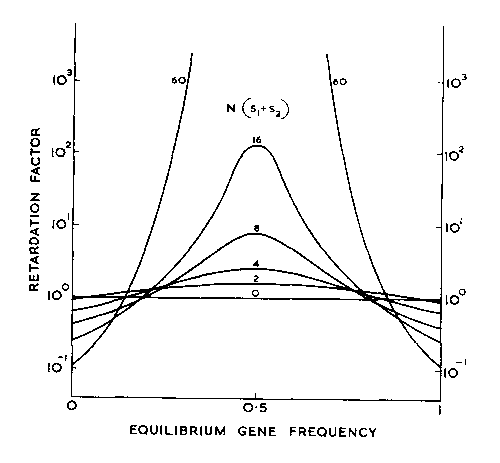
\includegraphics{drift-heterozygote-advantage.eps}}
\end{center}
}

\myslide{
\heading{Genetic draft}
\begin{center}
\resizebox{!}{0.9\textheight}{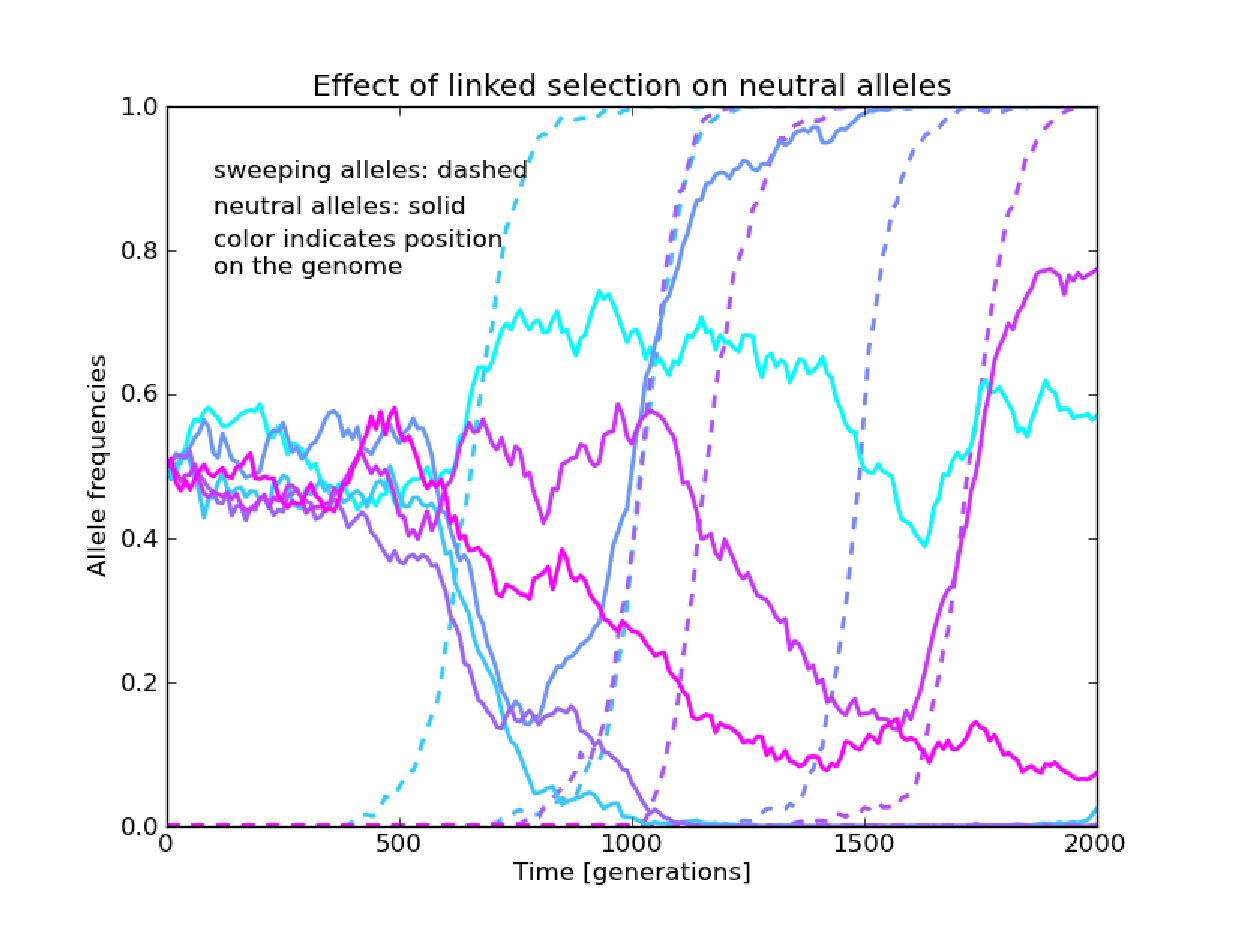
\includegraphics{genetic-draft.eps}}
\end{center}
}

\myslide{
\begin{center}
\resizebox{\textwidth}{!}{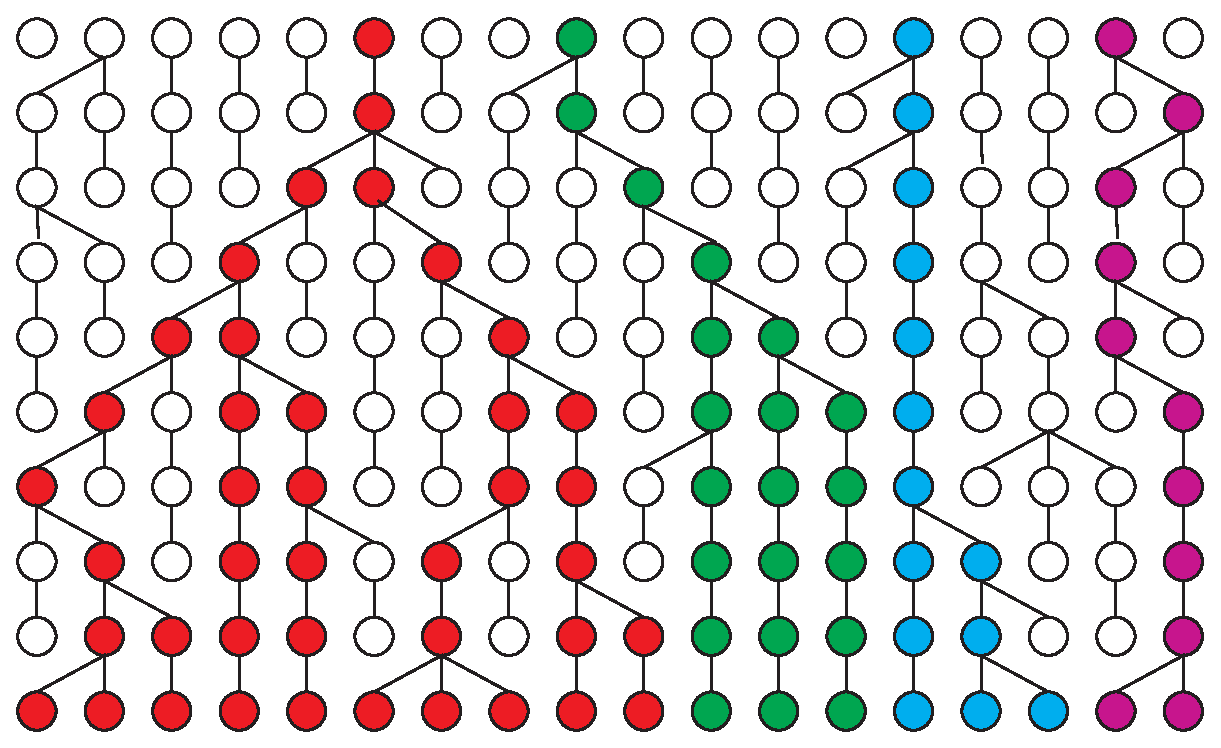
\includegraphics{coalescent-figure.eps}}
\end{center}
}

\myslide{
\heading{Kingman's coalescent (two allele copies)}

\[
\mbox{P}(\hbox{two alleles ibd}) = \frac{1}{2N_e^{(f)}}
\]
\vfill
\[
\mbox{P}(\hbox{coalescent at time $t$} = \left(1 - \frac{1}{2N_e}\right)^{t-1}\frac{1}{2N_e}
\]
\vfill
\[
\hbox{Average time to coalescence of two alleles} = 2N_e
\]
}

\myslide{
\heading{Kingman's coalescent (multiple allele copies)}

\begin{eqnarray*}
m &=& \hbox{number of allele copies} \\
\hbox{number of allele copy pairs} &=& \frac{m(m-1)}{2} \\
\mbox{P}(\hbox{coalescent involving one pair of alleles}) &=& 
\left(\frac{m(m-1)}{2}\right)\left(\frac{1}{2N_e}\right) \\
\hbox{Average time to coalescent event} &=&
\left(\frac{2}{m(m-1)}\right)\left(2N_e\right) \\
&=& \frac{4N_e}{m(m-1)} 
\end{eqnarray*}
}

\myslide{
\heading{Kingman's coalescent (multiple allele copies)}

\begin{eqnarray*}
\hbox{Average time to coalescent event} &=& \frac{4N_e}{m(m-1)} 
\end{eqnarray*}
Now there are $m-1$ alleles
\begin{eqnarray*}
\hbox{Average time to next coalescent event} &=& \frac{4N_e}{(m-1)(m-2)} 
\end{eqnarray*}
\vfill
\begin{eqnarray*}
\bar t &=& \sum_{k=2}^m \frac{4N_e}{k(k-1)} \\
       && \mbox{TAMO} \\
       &=& 4N_e\left(1 - \frac{1}{m}\right) \\
       &\approx& 4N_e
\end{eqnarray*}
}

\myslide{
\heading{Mitochondrial Eve}

Data
\begin{itemize}

\item Mitochondrial DNA from 147 humans

\item Most recent common ancestor 200,000 years ago

\end{itemize}

Expectation
\begin{itemize}

\item All mitochondrial genomes share a single common ancestor $2N_e$
  generations ago.

\item Human generation time $\approx$ 20 years. 

\item 200,000 years $\approx$ 10,000 generations.

\item Coalescence of all mitochondria consistent with $N_e$ of 5000.

\end{itemize}
}

\myslide{
\heading{Coalescent in structured populations}

{\small
\begin{eqnarray*}
\bar t_0 &=& \mbox{average time to coalescence of allele copies from
             the same population} \\
\bar t_1 &=& \mbox{average time to coalescence of allele copies from
             different populations} \\
\bar t &=& \mbox{average time to coalescence of allele copies} \\
       &=& \frac{k(k-1)\bar t_1 + k\bar t_0}{k^2}
\end{eqnarray*}
}
\vfill
If mutation is rare,
\[
F_{st} = \frac{\bar t - \bar t_0}{\bar t} \quad .
\]
}

\end{document}



\end{document}



